\documentclass[a5paper, DIV=18, 12pt]{scrartcl}
\usepackage{recycle}
\usepackage{multicol}
\setlength\columnsep{0.75cm}
\usepackage{enumitem}
\usepackage[margin=0.925cm]{geometry}


\usepackage{fontspec}
\usepackage[dvipsnames]{xcolor}
\usepackage{tikz}
\setmainfont[Scale=1.0]{Tex Gyre Schola}
\usepackage{eso-pic}

\setkomafont{section}{\setmainfont[Scale=1.125]{Tex Gyre Schola-Bold}\LARGE}
\setkomafont{subsection}{\setmainfont{Tex Gyre Schola-Bold}\Large}
\setkomafont{subsubsection}{\setmainfont{Tex Gyre Schola-Bold}\large}

\usepackage{contour}
\contournumber{32}
\usepackage[letterspace=0]{microtype}


% Adjust spacing before and after section headings
\RedeclareSectionCommand[
  runin=false,
  beforeskip=0.75\baselineskip,
  afterskip=0.5\baselineskip
]{section}

% Adjust spacing before and after subsection headings
\RedeclareSectionCommand[
  runin=false,
  beforeskip=0.5\baselineskip,
  afterskip=0.5\baselineskip
]{subsection}

% Adjust spacing before and after subsubsection headings
\RedeclareSectionCommand[
  runin=false,
  beforeskip=0.5\baselineskip,
  afterskip=0.5\baselineskip
]{subsubsection}

\colorlet{permred}{Red}
\colorlet{permyellow}{Goldenrod}
\colorlet{permgreen}{LimeGreen}
\colorlet{permblue}{RoyalBlue}

\newcommand{\cc}[2]{\contour*{black}{\textcolor{#1}{#2}}}

\newlength{\klen}
\setlength{\klen}{0em}%{0.125em}

\pagestyle{empty}
\raggedright
\begin{document}
%\AddToShipoutPictureBG{
%\begin{tikzpicture}[remember picture, overlay]
%	\node[opacity=0.25] () at (current page.center) {
\includegraphics[width=\pagewidth, height=\pageheight]{Images/newspaper_background2b_a4.jpg}};
%\end{tikzpicture}
%}
\phantom{a}
\enlargethispage{1\baselineskip}
\vspace{-4ex}
{
\begin{center}
\setmainfont[Scale=1.9475]{Digital Geometric-Light}\Huge \cc{permred}{P}\kern \klen\cc{permblue}{e}\kern \klen\cc{permyellow}{r}\kern \klen\cc{permgreen}{m}\kern \klen\cc{permyellow}{u}\kern \klen\cc{permblue}{t}\kern \klen\cc{permgreen}{a}\kern \klen\cc{permyellow}{t}\kern \klen\cc{permred}{i}\kern \klen\cc{permgreen}{o}\kern \klen\cc{permred}{n}\kern \klen\cc{permblue}{s}
\end{center}
}

\vspace{1ex}


\includegraphics[scale=0.125]{Images/Icons/player_count_icon.png} {\setmainfont[Scale=1.4]{Tex Gyre Schola-Bold}\Huge \raisebox{6.55pt}{\textcolor{black}{:\ 2-5}}} \hfill 
\includegraphics[scale=0.125]{Images/Icons/player_age_icon.png} {\setmainfont[Scale=1.4]{Tex Gyre Schola-Bold}\Huge \raisebox{6.55pt}{\textcolor{black}{:\ 8+}}}\hfill 
\includegraphics[scale=0.125]{Images/Icons/playtime_icon.png} {\setmainfont[Scale=1.4]{Tex Gyre Schola-Bold}\Huge \raisebox{6.55pt}{\textcolor{black}{:\ 30}}}
\vspace{-0.25ex}
\flushleft
\begin{center}{\setmainfont[Scale=1.0]{Tex Gyre Schola}A lightweight game that combines satisfying, snappy card play\\with the suspense and excitement of sealed-bid auctions.}
\end{center}
\vspace{-1ex}

\section*{\phantom{a}\hfill Bidding \& Collecting \hfill \phantom{a}}
\begin{multicols}{2}\itshape
It's an auction, place your bids!

\vspace{1ex}

Remember, high bidders get to collect their cards first.

\vspace{1ex}

Which card do you want? 

\vspace{0.9ex}

Choose wisely! Your score depends on the colours and icons on the cards you collect.

\vspace{0.9ex}

Remember, too, that you will use the cards you collect now to make your bids next round.

\vspace{0.9ex}

Will you take a star card for some guaranteed points? 

\vspace{0.9ex}

Or, will you take a high card for future bidding power?
\normalshape
\vfill\null

\vfill

\begin{center}
%\phantom{a}
%
%\vspace{-0.75ex}


\includegraphics[width=0.225\textwidth]{Images/single_display_card_40.pdf} \hfill 
\includegraphics[width=0.225\textwidth]{Images/single_display_card_10.pdf} 

\vspace{1.0ex}

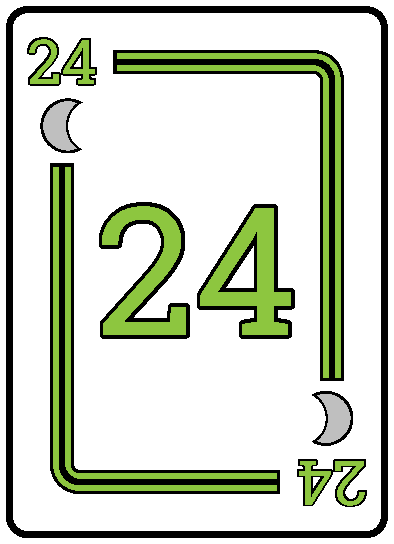
\includegraphics[width=0.225\textwidth]{Images/single_display_card_24.pdf} \hfill 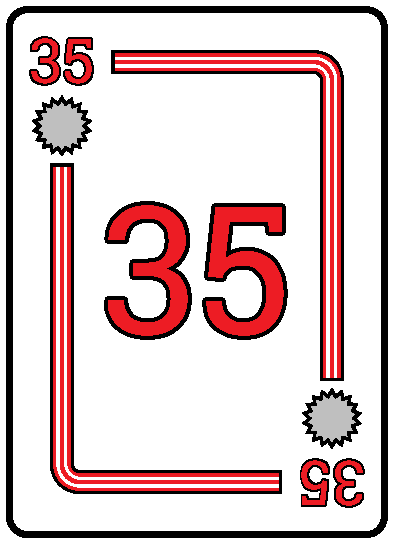
\includegraphics[width=0.225\textwidth]{Images/single_display_card_35.pdf} 
\end{center}

\vfill\null
\end{multicols}

\vspace{-7ex}

%\begin{multicols}{2}
\section*{\phantom{a}\hfill Components \& Features\hfill \phantom{a}}
\begin{itemize}[leftmargin=*, nosep]
\item \hspace{0.05pt}Fifty double-suited cards create a rich decision space.  
\vspace{0.4ex}
\item Auctions provide tough choices and tense resolutions.
\vspace{0.4ex}
\item Simultaneous bidding minimises downtime.
\vspace{0.4ex}
%\item Simple scoring rewards clever, tactical gameplay.
\item Tactical gameplay keeps players engaged from start to finish.
%\vspace{0.4ex}
%\item The best part is, it's always your turn!
\end{itemize}
\vfill


\begin{center}
\textbf{Design}: Michael Purcell \hfill \textbf{Contact:} mike@armiger.games
\end{center}

\end{document}